%!TEX program = xelatex

\documentclass[a4paper, twocolumn]{ctexart}

% layout
\usepackage{abstract}
\usepackage{fancyhdr}
\usepackage{flushend}
\usepackage[scale=0.8]{geometry}
% content
\usepackage{authblk}
\usepackage{biblatex}
\usepackage{graphicx}
\usepackage{hyperref}
\usepackage{mathtools}

\pagestyle{fancy}

\addbibresource{reference.bib}

\title{对种群动态的数学手段模式化分析方法建立暨对实际农作物生产场景预测分析}
\author{马宜远}
\author{孙嘉俊}
\author{王明哲 \thanks{通讯作者}}
\renewcommand \Authands{,}
\affil{大连第二十四中学}
\date{}

\begin{document}

\twocolumn[
    \maketitle
    \strong{摘要}：
    生态学在农业生产中常被用于预测农作物产量.
    本文使用计算机分析方法,
    就不同生态因素对叶菜类农作物产量影响进行建模,
    得到了综合种内、种间竞争、天敌影响、土壤肥力等生态因素综合作用下的叶菜类农作物种群数量模型,
    最终得以精准预测、精准干预.

    \strong{关键词}：农作物产量预测；计算机模拟；生态学模型

    \vspace{1cm}
]
\saythanks

农业是我国的基础产业,在我国有着悠久的历史.
新中国成立后,我国人口迅速增长,
但受客观因素影响,我国存在人均占有耕地面积少、耕地品质不足等问题,
农业产能难以满足人口增长的需要.
农业生产中,作物的产量往往是人们亟需关注的问题.
在高中生物选修二《种群的数量特征》中,
我们初步学习了“J形增长曲线”与“S形增长曲线”,
即指数增长曲线与逻辑斯蒂曲线.
为进一步深入、系统地学习,并应用到实际生活中,
我们开展了本次研究,结合生态学知识与信息技术,
将实际生产中难以量化计算的生态学因素,
使用数学语言精确表达,建立数学模型,并使用计算机进行数值分析.
考虑到农业的经济效益影响,我们选择叶菜类农作物进行建模,
并结合现实环境因素进行模拟.

\section{常见生态学模型}

\subsection{Logistic 增长模型}

\subsubsection{简述}
皮埃尔-弗朗索瓦·韦吕勒（P.F.Verhulst, 1804-1849）于 1838 年提出
\strong{Logistic 增长模型} \autocite{logistic_origin},
对应方程称为 Logistic 方程,
为描述资源有限环境下种群增长的最简单模型,
也是多数生态学模型的基础.
我们熟知的“S形增长曲线”即为该模型.

\subsubsection{数学模型描述}
由于生境中资源有限,考虑引入环境对种群的影响,
可使用比值$\frac{K - N}{K}$限制种群增长,
并添加常数$r$以控制增长速率.如此,可以得到
\begin{equation} \label{eq:logistic}
    \boxed{\frac{\mathrm{d} N}{\mathrm{d} t} = r N (1 - \frac{N}{K}).}
\end{equation}

其中$N$为种群数量,$t$为时间,
$K$为生物的\strong{环境容纳量(environmental capacity)},
$r$为\strong{内禀增长率(innate rate of increase)}.
内禀增长率$r$是一个经验数值,可由近似公式
\begin{equation*}
    r = \frac{\ln R_0}{T}
\end{equation*}
给出.
其中$R_0$为净生殖率,即一个世代中种群的增长倍数,$T$为世代时间.

式 \eqref{eq:logistic} 为一阶常微分方程,通解为
\begin{equation*}
    N_t = \frac{K}{1 + (\frac{K}{N_0} - 1) e^{-r t}},
\end{equation*}
函数图像如图\ref{fig:logistic}所示.
\newline

\begin{figure}[h]
    \centering
    
\includegraphics[width=\columnwidth]{./figures/logistic.pdf}
    \caption{Logistic 增长模型}
    \label{fig:logistic}
\end{figure}

Logistic 方程十分简洁,但未考虑种间影响.
接下来,我们将在逻辑斯蒂增长模型的基础上,增加种间竞争的因素.

\subsection{Lotka-Volterra 竞争模型}

\subsubsection{简述}
二十世纪 20-30 年代,艾尔弗雷德·洛特卡(Alfred Lotka, 1880-1949)
独立提出了描述种间竞争的简单数学模型,即\strong{Lotka-Volterra 竞争模型},
为生态学中描述种间竞争的基本模型.

\subsubsection{数学模型描述}
生物竞争的本质是对有限资源的争夺.
考虑种群之间的生境重叠,
可使用$\frac{N_j}{K_i}$描述第$j$种群对第$i$种群生境的占据作用.

考虑两个种群的竞争
\begin{subequations} \label{eq:lv-comp:part}
    \begin{align}
        \frac{\mathrm{d} N_1}{\mathrm{d} t} = r_1 N_1 (1 - \frac{N_1}{K_1} - \alpha_{1,2} \frac{N_2}{K_1}), \\
        \frac{\mathrm{d} N_2}{\mathrm{d} t} = r_2 N_2 (1 - \frac{N_2}{K_2} - \alpha_{2,1} \frac{N_1}{K_2}).
    \end{align}
\end{subequations}

与方程\eqref{eq:logistic}相比,
方程\eqref{eq:lv-comp:part}仅添加$\alpha_{i,j} \frac{N_j}{K_i}$一项（简称为“竞争项”）,
其中$\alpha_{i,j}$为\strong{竞争系数(coefficient of competition)},
描述\strong{第$j$种群对第$i$种群的竞争程度}.

\begin{figure}[h]
    \centering
    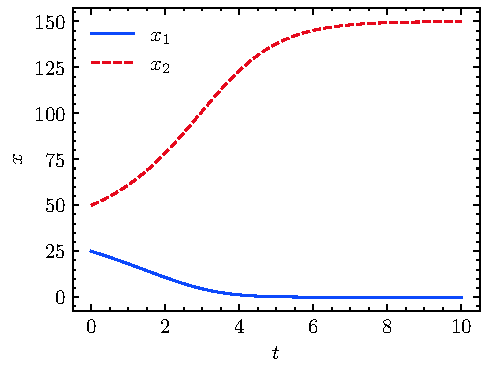
\includegraphics[width=\columnwidth]{./figures/lotka-volterra-competition.pdf}
    \caption{Lotka-Volterra 竞争模型}
    \label{fig:lv-comp}
\end{figure}

更一般地,若存在多个种群,则可叠加不同种群间的竞争项
\begin{equation} \label{eq:lv-comp}
    \boxed{\frac{\mathrm{d} N_i}{\mathrm{d} t} = r_i N_i (1 - \frac{1}{K_i} \sum_{j} \alpha_{i,j} N_j).}
\end{equation}

方程\eqref{eq:lv-comp}将 Logistic 方程\eqref{eq:logistic}中$\frac{N_i}{K_i}$一项并入求和,
既是为了保持方程形式简洁,也为引入\strong{竞争系数的矩阵表示}提供方便.

\subsubsection{竞争系数的矩阵表示}
如前文所述,竞争系数$\alpha_{i,j}$描述第$j$种群对第$i$种群的竞争程度.
注意到这里若要指定具体的$\alpha_{i,j}$,需要$i$, $j$两个值,
若种群数量为$n$,则竞争系数共有$n^2$个.
随种群数量$n$增长,大量系数若采用列表表示,将难以维护.

此时可以令$i$,$j$分别表示行索引与列索引,构造一个$n \times n$\strong{矩阵(matrix)}
\begin{equation*}
    \alpha := \begin{bmatrix}
        \alpha_{1,1} & \alpha_{1,2} & \cdots & \alpha_{1,j} & \cdots & \alpha_{1,n} \\
        \alpha_{2,1} & \alpha_{2,2} & \cdots & \alpha_{2,j} & \cdots & \alpha_{2,n} \\
        \vdots & \vdots & \ddots & \vdots & \ddots & \vdots \\
        \alpha_{i,1} & \alpha_{i,2} & \cdots & \alpha_{i,j} & \cdots & \alpha_{i,n} \\
        \vdots & \vdots & \ddots & \vdots & \ddots & \vdots \\
        \alpha_{n,1} & \alpha_{n,2} & \cdots & \alpha_{n,j} & \cdots & \alpha_{n,n}
    \end{bmatrix},
\end{equation*}
如此便能方便地表示竞争系数.
\newline

Lotka-Volterra 竞争模型描述了种间竞争关系.
接下来,我们将进一步引入捕食关系.

\subsection{Lotka-Volterra 捕食模型}
% TODO: Lotka-Volterra predation

\subsubsection{简述}

\subsubsection{食草动物的引入}
现在我们把食草动物引入这一模型,只需在原方程上额外增加一项,
以表达受食草动物的啃食程度,因此方程可以写为
\begin{equation}
    \frac{\mathrm{d} V}{\mathrm{d} t} = r_m (1 - \frac{V}{K}) - c_1 H (\frac{1 - e^{-d_1} V}{V})
\end{equation}

其中,$H$代表食草动物种群的生物量,
$c_1$代表食物充足情况下每个食草动物单位的最大食物摄取率.
当$V$减少时,动物便不再能充分取食,
$c_1$便以$v_1 := 1 - e^{-d_1} V$的速率下降,
当$V \rightarrow 0$时,$v_1 \rightarrow 1$.
$d_1$为常数,决定下降率,同时也表示食草动物的取食效率.
可见,对食草动物来说,$c_1 v_1$就相当于捕食动物的功能反应,
用以表示食草动物摄取率对食物量变化所发生的反应.
可以推导食草动物种群的增长率
\begin{equation}
    \frac{\mathrm{d} H}{\mathrm{d} t} = a_2 + c_1 (1 - e^{d_1} V)
\end{equation}

\subsubsection{食肉动物的引入}
如果把捕食动物猎杀食草动物引入上述模型,模型就会变得更加复杂.
其中的植物种群方程仍然保持不变,但描述食草动物增长的方程会因为加入
食肉动物而变得复杂起来
\begin{equation}
    \frac{\mathrm{d} H}{\mathrm{d} t} = a_2 + c_2 (1 - e^{d_2} V) - f P (\frac{1 - e^{-d_3} H}{H})
\end{equation}

对于食肉动物,我们则采用一个新方程加以描述
\begin{equation}
    \frac{\mathrm{d} P}{\mathrm{d} t} = -a_3 + c_3 (1 - e^{d_4} H)
\end{equation}

这样一个模型虽然仍然简陋,
但已经可以对叶菜类农作物的产量做出初步的预测和较为准确的判断,
尤其表现出了产量变化的逐步过程,这对于农业生产也是极其重要的.

\section{计算机模拟对实际应用的结合}

\subsection{数学与农田的对话}
数学建模作为现实生活中的一个重要工具,
它用简洁的数学语言描述了事物的变化.
在理解种群动态的任务中,尤其是从理论模型到实际应用的场景,
我们仍然面对诸多挑战.

\subsection{计算机模拟结果对实际应用的作用}

\subsubsection{预见性}
原始的农业生产在有限的经验下,
需要克服不确定的气候、资源等因素,才能提升产量.
计算机的模拟可以使经验判断成为定量计算.
值得注意的是,这种预见性并不要求模型的绝对准确.
复杂计算机模型的校准需要明确处理结构的误差——意识到模型只是对现实的近似,
结果本身包含一定误差,这对决策者而言也是非常重要的信息.

\subsubsection{优化性}
如上文所述,模型只是对现实的近似.
显而易见,模型越逼近现实,其实用价值越高.
计算机模拟与优化算法的结合,为解决这类问题提供了可行路径.
优化算法可以自我改进深度优化算法,探索许多人类无法察觉的微小因素,
从而做出更加精准的判断.

\subsubsection{普及性}
理想情况下,每一个农民都要掌握一定的气象、经济学知识,
能准确解读天气数据,能优化资源配置,但现实不是这样的.
计算机模拟在降低专业知识应用门槛方面可以发挥独特作用.
农民不必理解模型内部的微分方程,不必掌握编程技能就能获得准确可靠的数据.

\section{结论与展望}
数学建模与计算机模拟的价值,终究要由实践来检验.
在这个意义上,模型永远只是模型——是对现实的简化与近似.
但这种简化如果得当,
就能帮助我们从复杂中识别简单,从噪声中辨别信号,从不确定性中锚定决策.
这或许正是“对种群动态的数学手段模式化分析”对农作物生产场景的最根本贡献.
当然了,我们也要看到研究的局限性.
从空间的角度看,如在 LV 竞争模型中,如果我们拥有一个更加广阔的充足空间,
就需要考虑到种群的空间分布对于其数量变化的影响.
例如大型食肉动物对小型动物的威慑作用.
从时间的角度看,因其还不具备引入长期复杂现实因素的能力,
可能在更加广阔的时间尺度上略显逊色.
例如将时间线拉长,我们可能要考虑到进化、演替等因素,
以及基因的变异、自然选择等等.
短期内这些因素不会对模拟结果造成太大影响,
但是当时间线拉长,它们对于预测结果的影响程度成指数级增加,
成为我们不能忽略不计的因素.
从社会的角度看,计算机模拟的能力仍然不足.
从人类影响的程度上看,就本研究的例子而言,当我们进一步思考实际意义,
我们需要考虑到人工对害虫的扑杀等因素.
人类对自然的影响是丰富的,不仅仅体现在程度上,更体现在形式上.
每一个人的细微举动都会对自然造成影响,
当人流量增大,如在考虑人口增长或是城市中公园的生态问题时,
这些影响也是不可忽略的因素.
而计算机如何体现各种各样形式的影响成为了我们面对此类问题时的主要挑战.
数学建模与计算机模拟的价值,终究要由实践来检验.
在这个意义上,模型永远只是模型——是对现实的简化与近似.
但这种简化如果得当,
就能帮助我们从复杂中识别简单,从噪声中辨别信号,从不确定性中锚定决策.
这或许正是“对种群动态的数学手段模式化分析”对农作物生产场景的最根本贡献.
我们相信在不远的将来,
计算机技术可以成熟的被运用到实际生产生活当中,让人类的生活更加美好.

\printbibliography[title=参考文献]

\end{document}
